\documentclass{article}
\usepackage[utf8]{inputenc}
\usepackage[spanish]{babel}
\usepackage{blindtext}
\usepackage{outlines}
\usepackage{authblk}
\usepackage{multicol}
\usepackage{geometry}
\usepackage{amssymb}
\usepackage{tabto}
\usepackage{biblatex}
\usepackage{graphicx}
\graphicspath{ {images} }
\addbibresource{ed.bib} %Import the bibliography file
 \geometry{
 letterpaper,
 left=25mm,
 top=25mm,
 bottom=25mm,
 right=30mm
 }
\title{ Solución de la ecuación diferencial: general y particular. Definición de solución singular.}
\author{Jorge Ruiz López}
\affil{Facultad de Ingeniería UNAM}
\date{March 2022}
\begin{document}
\maketitle
\section{Solución de una ecuación diferencial:}
\begin{description}
\item[Definición 1.1:]\textbf{Solución}\cite{carmona} de una ecuación diferencial es una función que no contiene derivadas y que satisface a dicha ecuación; es decir, al sustituir la función y sus derivadas en la ecuación diferencial resulta una identidad.
\item[Definición 1.2:]\textbf{Solución general} de una ecuación diferencial es la función
que contiene una o más constantes arbitrarias (obtenidas de las sucesivas integraciones).\\
\textbf{Ejemplo:} La función $x+y^2 = c$ es la \emph{solución general} de la ecuación diferencial:
\begin{center} $\frac{dy}{dx} = -\frac{1}{2y}$ \end{center}
Porque derivándola implícitamente tenemos: $1+2y\frac{dy}{dx} = 0$, o expresado en otra forma: $2yy' = -1$.
Sustituyendo y y y' obtenemos una identidad: 
\begin{center}${2\sqrt{c-x}} {(-\frac{1}{2\sqrt{c-x}})} = -1$ $\blacksquare  -1 = -1$;\\
donde $y=\sqrt{c-x}$\end{center}
\textbf{Ejemplo 2:} La función $y=3x^2+c_1x+c_2$ es \emph{solución general} de la ecuación diferencial $y''= 6$, porque \begin{center}$y'=6x +c_1$\\ y $y'' = 6$ $\blacksquare 6=6$\end{center}
\item[Definición 1.3:]\textbf{Solución particular} de una ecuación diferencial es la función cuyas constantes arbitrarias toman un valor específico.\\
\textbf{Ejemplo:} La función $y = e^{-x}+8$ es \emph{solución particular} de la ecuación diferencial 
$y'+e^x=0$, porque derivando la solución y sustituyéndola en la ecuación dada, obtenemos:
\begin{center}
$y'=-e^{-x}$\\$-e^{-x}+e^{-x}=0$ $\blacksquare 0 = 0$
\end{center}
\item[Definición 1.4: Solución singular] de una ecuación diferencial es una función cuya tangente a su gráfica en cualquier punto $(X_0, Y_0)$ coincide con la tangente de otra solución, pero ya no coincide con esta última tangente en ninguna vecindad del punto $(X_0, Y_0)$, por pequeña que ésta sea.\\\\
Estas soluciones se obtienen a partir de la solución general. Un método para encontrar dichas soluciones es derivar la ecuación diferencial dada con respecto a $y'$, con lo cual formamos un sistema de ecuaciones:\\
\begin{center}$F(x,y,y') = 0$ \\\break $\frac{\partial F(x,y,y')}{\partial y'} = 0$ \end{center}
del cual, eliminando $y'$, se obtienen una o más soluciones singulares.\\
\textbf{Ejemplo:} Hallar las soluciones singulares, si las hay, de la ecuación diferencial:\\
\begin{center}$y'^{2} = 16x^2$\end{center}
Derivando con respecto a $y'$, tenemos:\\
\begin{center}$2y' = 0$\end{center}
De donde $y' = 0;$ sustituyendo en la ecuación, obtenemos $x = 0$, que es la solución singular.
En efecto, las soluciones generales de dicha ecuación son:
\begin{center}$y=2x^2+c$, $y=-2x^2+c$, \end{center}
y para el punto $(0,0)$ su gráfica es $y = \pm2x^2$\\
\begin{center}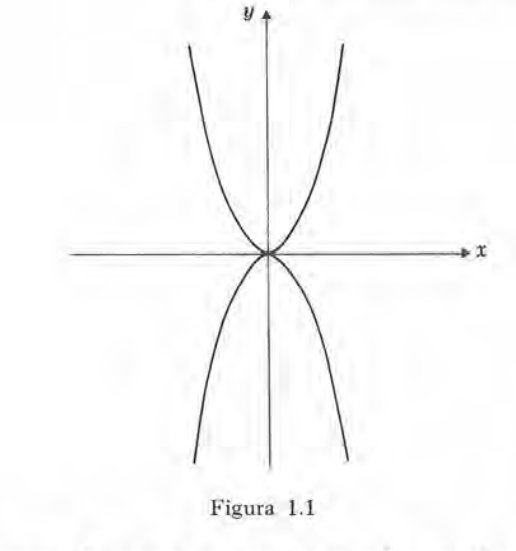
\includegraphics[scale=.55]{ed_sol_cingular.PNG}\end{center}
Y $x = 0$ es el punto de contacto con las pendientes de $y = \pm2x^2$ en el punto $(0,0)$.
\end{description}
\printbibliography
\end{document}
